% 大学物理实验报告

\documentclass[UTF8]{ctexart}

\usepackage{amsmath}        %数学公式
\usepackage{cases}          %联立编号
\usepackage{cite}           %引用
% \usepackage{enumitem}       %编号

\usepackage{graphicx}       %插入图片
\usepackage{float}          %设置图片浮动位置
\usepackage{subfigure}      %插入多图时用子图显示

\usepackage{anyfontsize}    %解决一个奇怪的字体大小报错问题
\usepackage{fancyhdr}       %页眉、页脚、页码
\usepackage[a4paper, margin=1in]{geometry}    %纸张大小

\newcommand\f[2]{\frac{#1}{#2}}
\newcommand\pf[2]{\frac{\partial#1}{\partial#2}}
\newcommand\df[2]{\dfrac{#1}{#2}}
\newcommand\pdf[2]{\dfrac{\partial#1}{\partial#2}}
\newcommand\zsin[1]{\frac{e^{i#1}-e^{-i#1}}{2i}}
\newcommand\zdsin[1]{\dfrac{e^{i#1}-e^{-i#1}}{2i}}
\newcommand\zcos[1]{\frac{e^{i#1}+e^{-i#1}}{2i}}
\newcommand\zdcos[1]{\dfrac{e^{i#1}+e^{-i#1}}{2i}}
\newcommand\zline[1]{#1-\overline{#1}}

\newcommand\dg[2]{#1^{\circ}#2'}

\setlength{\headheight}{16pt}
\pagestyle{fancy}
\fancyhf{}


\title{偏振光学实验}
\author{\LaTeX\ by\ Jerry\ }
\date{\today}
\pagenumbering{arabic}

\begin{document}

\fancyhead[L]{Jerry}
\fancyhead[C]{偏振光学实验}
\fancyfoot[C]{\thepage}

\maketitle
\tableofcontents
\newpage

\section{数据处理}

\subsection{观察激光束的偏振特性}

在起偏器$P$后放置一白纸屏,转动起偏器,观察激光器光源经起偏器$P$后的强度变化。

记录光强极小时起偏器的度盘读数:$40.8^{\circ}$、$221.8^{\circ}$。

将起偏器转至光强较强的角度。

\subsection{观测布氏角}

\textbf{原理:}光束以布儒斯特角入射时,反射光为电矢量垂直于入射面的完全线偏振光,反射光中没有电矢量与入射面平行的分量。如起偏器透射轴在水平方向,则入射光电矢量与入射面平行,反射光强极小。

\textbf{方法:}使激光束以布儒斯特角入射反射镜表面,调整起偏器$P$方位角,当反射光强极小时,则起偏器$P$的透射轴位于水平方向。

\textbf{步骤:}

1)测量光束正入射反射镜表面时的平台方位角:将反射镜放在小平台上,自制带小孔的纸片放置在出射光束处,调整小平台使反射光束与激光器出射光束重合,记录此时的平台方位角$\alpha_{i=0}=\dg{121}{4}$

2)观测布儒斯特角、定起偏器$P$透射轴方向:转动小平台,使反射光束朝向实验者自身(反射光束禁止向照射他人方向转动),并使入射角约为55°。用白纸屏观测光强。交替调整小平台(即入射角)和起偏器$P$方位角,使反射光强极小。记录此时的小平台方位角和起偏器$P$方位角(应与任务0的读数显著不同)。重复测量3次。测量数据记于表\ref{tab:1.2.1}。

\begin{table}[h]
    \centering
    \begin{tabular}{|c|c|c|}
        \hline
        序号 & 入射角为布儒斯特角时的平台方位角$\alpha_B$ & 起偏器$P$透射轴在水平方向的方位角$p$ \\ \hline
        1 & $\dg{247}{58}$ & $88.2^{\circ}$ \\ \hline
        2 & $\dg{247}{37}$ & $88.9^{\circ}$ \\ \hline
        3 & $\dg{247}{30}$ & $88.1^{\circ}$ \\ \hline
        平均值 & $\dg{247}{42}$ & $88.4^{\circ}$ \\ \hline
    \end{tabular}
    \caption{观测布儒斯特角数据}
    \label{tab:1.2.1}
\end{table}

Brewster角测量值$\theta_B=\dg{53}{22}$ ,折射率$n = \tan\theta_B = 1.34487$。

\subsection{定检偏器$A$的透射轴方向}

\textbf{原理:}起偏器$P$透射轴位于水平方位的方位角已确定,当检偏器$A$透射轴在垂直方向时,与起偏器$P$正交消光。

\textbf{步骤:}1)置起偏器$P$方位角于$p_{\leftrightarrow}$测量平均值位置;2)移去反射镜;3)用毫伏表测量光强;4)转动检偏器$A$使其与起偏器$P$正交消光,此时检偏器$A$的透射轴在垂直方向,记为$\alpha_{\updownarrow}=4.0^{\circ}$。

\subsection{测消光比$e$}

$P$盘不动,转动$A$盘,交替测透射光强极值$I_{max}$和$I_{min}$ (用mV表示)。测量数据记于表\ref{tab:1.4.1}。

\begin{table}[h]
    \centering
    \begin{tabular}{|c|c|c|}
    \hline
        测量次数 & $I_{max}$ (mV) & $I_{min}$ (mV) \\ \hline
        1 & 1.714 & 0.007 \\ \hline
        2 & 1.715 & 0.006 \\ \hline
        3 & 1.717 & 0.006 \\ \hline
        平均值 & 1.7153 & 0.0063 \\ \hline
    \end{tabular}
    \caption{消光比测量数据}
    \label{tab:1.4.1}
\end{table}

电阻箱阻值$R=100\Omega$

挡住光源时$I_0=0.006$mV

计算得到消光比$e = \dfrac{\overline {I_{min}} - I_0}{2I_{max}} =9.716\times10^{-5}$

\subsection{测量透射光强与两偏振器$P$与$A$之间夹角$\theta$的关系}

\textbf{原理:}起偏器$P$后的出射光束为线偏振光,设其光强为$I_{max}$,该线偏振光经检偏器$A$后,根据马吕斯定律,其出射光强为$I_{max}\cos^2\theta$。

\textbf{步骤:}起偏器$P$置于水平方向且保持不动,转动检偏器$A$至不同方位角,测量经检偏器$A$后出射光强。

电阻箱示值$R = 100 \Omega$,$P=\overline{P_{\leftrightarrow}}=88.4^{\circ}$,$\alpha_{\updownarrow} = 4.0^{\circ}$,挡住光源时 $I_0 = 0.006 $ mV

\begin{table}[h]
    \centering
    \begin{tabular}{|c|c|c|c|c|c|}
    \hline
        序 & 起偏器检偏器夹角 & $A$方位角 $\alpha=$ & 出射光强测量值 & 相对透过率 & $\cos^2\theta$ \\
        号 & $\theta$ (°) & $\alpha_{\updownarrow}+90+\theta$ (°) & $I_m$ (mV) & $(I_m- I_0)/ (I_{max}- I_0)$ & \\ \hline
        1 & 0.0 ($I_{max}$) & 94.0 & 1.718 & 1.0000 & 1.0000 \\ \hline
        2 & 15.0 & 109.0 & 1.606 & 0.9346 & 0.9330 \\ \hline
        3 & 30.0 & 124.0 & 1.294 & 0.7523 & 0.7500 \\ \hline
        4 & 45.0 & 139.0 & 0.869 & 0.5040 & 0.5000 \\ \hline
        5 & 60.0 & 154.0 & 0.434 & 0.2500 & 0.2500 \\ \hline
        6 & 75.0 & 169.0 & 0.120 & 0.0666 & 0.0699 \\ \hline
        7 & 80.0 & 174.0 & 0.060 & 0.0315 & 0.0302 \\ \hline
        8 & 84.0 & 178.0 & 0.027 & 0.0123 & 0.0109 \\ \hline
        9 & 87.0 & 181.0 & 0.012 & 0.0025 & 0.0027 \\ \hline
        10 & 90.0 ($I_{min}$) & 184.0 & 0.006 & 0.0000 & 0.0000 \\ \hline
    \end{tabular}
    \caption{透射光强与两偏振器$P$与$A$之间夹角$\theta$的关系}
    \label{tab:1.5.1}
\end{table}

画出相对透射率随$\theta$变化的关系曲线,并与理论值$\cos2\theta$的曲线相比较

\begin{figure}[h]
    \centering
    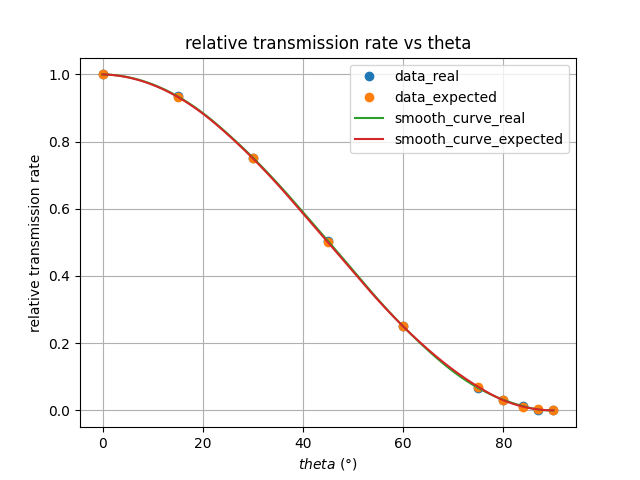
\includegraphics[width=0.8\textwidth]{img/relative_transmission_rate_vs_theta.png}
    \caption{透射光强与两偏振器$P$与$A$之间夹角$\theta$的关系}
    \label{fig:1.5.1}
\end{figure}

如图\ref{fig:1.5.1}(下一页)所示,实验数据与理论曲线几乎完全重合,可以认为符合较好,在给定的实验条件下马吕斯定律成立。

\subsection{定待测波片$C_X$的轴向}

\textbf{原理:}将待测波片放在已正交消光的起偏器$P$和检偏器$A$之间。旋转波片$C$,使三者仍保持消光状态,这时波片的一个轴就已平行于偏振器P的透射轴方向。

\textbf{步骤:}将起偏器$P$透射轴置于水平方向,$\overline{p_{\leftrightarrow}}= 88.4^{\circ}$,检偏器$A$透射轴置于垂直方向 $\alpha_{\updownarrow} = 4.0^{\circ}$。将待测波片$C_X$置于小平台上。转动待测波片$C_X$,使三者消光,记录待测波片$C_X$的一个轴在垂直方向时的度盘示值 $c_x = 177^{\circ}$。

\subsection{定波片$C_0$的快轴方向(大致方向已标出)}

\textbf{原理:}同上。

\textbf{步骤:}移去待测波片$C_X$。轻轻地装上仪器配套的波片盘$C_0$,用上一步骤方法定出波片快轴在垂直方向时的度盘方位角$c_0=196.8^{\circ}$。该波片快轴大致方向已在盘上用圆点标出。

\subsection{观测线偏振光经过1/4波片$C_0$后的偏振态的改变}

\textbf{内容:}观测线偏振光经过1/4波片$C_0$后的偏振态的改变。

\textbf{方法:}激光器经起偏器$P$后的出射光束为线偏振光。该线偏振光经过1/4波片$C_0$后,出射光的偏振态与波片和起偏器之间夹角$\beta$有关。通过检偏器$A$和光强计(毫伏表)可检验出射光的偏振态。

\textbf{步骤:}保持1/4波片$C_0$快轴于垂直方向,转动起偏器$P$,使起偏器$P$的透射轴与波片慢轴之间的夹角$\beta$分别为$0^{\circ}$、$22.5^{\circ}$、$45^{\circ}$、$67.5^{\circ}$。在每个夹角$\beta$处,转动检偏器$A$,测出透射光的长轴方位角$\alpha_i$和光强极大值$I_{\text{max}}$、极小值$I_{\text{min}}$。计算极值比。

起偏器$P$透射轴置于水平方向 $p_{\leftrightarrow} = 88.4^{\circ}$,波片$C_0$度盘示值 $c_0 = 196.8^{\circ}$。

\begin{table}[h]
    \centering
    \begin{tabular}{|c|c|c|c|c|c|c|c|c|c|}
        \hline
        序号 & $p-p_{\leftrightarrow}$ (°) & $p$ (°) & $\alpha_i$ (°) & $I_{\text{max}}$ (mV) & $I_{\text{min}}$ (mV) & $\Psi$ (°) & $b^2/a^2$ & $\delta_r$ ($^{\circ}$) & $\psi$ ($^{\circ}$) \\ \hline
        1 & 0 & 88.4 & 273.8 & 1.225 & 0.007 & -179.8 & 0.0057 & - & - \\ \hline
        2 & 22.5 & 110.9 & 268.2 & 1.724 & 0.295 & -174.2 & 0.1711 & 56.1213 & 27.9239 \\ \hline
        3 & 45 & 133.4 & 240.5 & 1.322 & 0.889 & -146.5 & 0.6725 & 无解 & 无解 \\ \hline
        4 & 67.5 & 155.9 & 190 & 1.176 & 0.248 & -96 & 0.2109 & 无解 & 无解 \\ \hline
    \end{tabular}
    \caption{观测线偏振光经过1/4波片后的偏振态的改变实验数据}
    \label{tab:1.7.1}
\end{table}

其中,计算$\delta_r$和$\psi$的公式为:

\begin{equation}
    \delta_r = \arcsin\left(\frac{2\cdot \sqrt{I_{\text{min}}/I_{\text{max}}}}{\sin(2\beta)(1+I_{\text{min}}/I_{\text{max}})}\right)
\end{equation}

\begin{equation}
    \psi = \frac{1}{2}\arctan(\tan(2\beta)\cdot\cos\delta)
\end{equation}

可以看出,在$\beta=0^{\circ}$时,$I_{\text{min}}/I_{\text{max}}=0$,近似为线偏光;在$\beta=22.5^{\circ}\ \&\ 67.5^{\circ}$时,是椭圆偏振光,在$\beta=45^{\circ}$时,近似为圆偏振光。

\subsection{线偏振光通过1/2波片或全波片}

\textbf{内容:}令$C_0$的快轴和$C_x$的一轴平行。将起偏器$P$透射轴置于不同方位,观测起偏器$P$后出射的线偏振光经两波片后偏振态的改变(用检偏器$A$和毫伏表检验)。

$C_x$某轴置于垂直方向,度盘示值 $177^{\circ}$;$C_0$快轴置于垂直方向,度盘示值 $196.8^{\circ}$。

\begin{table}[h]
    \centering
    \begin{tabular}{|c|c|c|c|c|c|}
    \hline
        序号 & $p-p_{\leftrightarrow}$ (°) & $p$ (°) & $\alpha_i$ (°) & 光强读数 & $\alpha_{\updownarrow}-\alpha_i$ (°) \\
        \hline
        1 & 0.0 & 88.4 & 4.0 & 0.010 & 0.0 \\ \hline
        2 & 15.0 & 103.4 & 348.5 & 0.014 & -344.5 \\ \hline
        3 & 30.0 & 118.4 & 332.6 & 0.026 & -328.6 \\ \hline
        4 & 45.0 & 133.4 & 316.2 & 0.034 & -312.2 \\ \hline
    \end{tabular}
    \caption{线偏振光组合波片后偏振态的改变实验数据}
    \label{tab:1.9.1}
\end{table}

根据表格可以看出:此时波片特性为全波片,$C_X$的快轴为水平。

\subsection{线偏振光通过全波片或1/2波片}

\textbf{内容:}令C0的慢轴和Cx的同一个轴平行,观测线偏振光经过这两个1/4波片后偏振态的改变情况。

$C_x$某轴保持垂直方向不变,度盘示值 $177^{\circ}$;$C_0$快轴转动$90^{\circ}$至水平方向,度盘示值 $106.8^{\circ}$。

\begin{table}[h]
    \centering
    \begin{tabular}{|c|c|c|c|c|c|}
    \hline
        序号 & $p-p_{\leftrightarrow}$ (°) & $p$ (°) & $\alpha_i$ (°) & 光强读数 & $\alpha_{\updownarrow}-\alpha_i$ (°) \\
        \hline
        1 & 0.0 & 88.4 & 4.0 & 0.010 & 0.0 \\ \hline
        2 & 15.0 & 103.4 & 27.5 & 0.039 & -23.5 \\ \hline
        3 & 30.0 & 118.4 & 36.0 & 0.058 & -32.0 \\ \hline
        4 & 45.0 & 133.4 & 53.3 & 0.073 & -49.3 \\ \hline
    \end{tabular}
    \caption{线偏振光组合波片后偏振态的改变实验数据}
    \label{tab:1.10.1}
\end{table}

根据表格可以看出:此时波片特性为半波片,$C_X$的快轴为竖直。

\newpage
\section{思考题}

\subsection{如何由几个相同的 1/4 波片构成 1/2 波片和全波片}

将多个 1/4 波片以不同的方式堆叠在一起即可:

\begin{enumerate}
    \item 构成 1/2 波片:将两个相同的 1/4 波片以平行于它们的慢轴的方式堆叠在一起。
    \item 构成全波片:将四个相同的 1/4 波片以相互垂直的方式堆叠在一起。
\end{enumerate}

\subsection{如何判断波片是 1/2 波片和全波片}

可以通过计算波片的相位延迟来确定它的类型,观察相位可以由已知偏振方向的线偏光在通过组合波片后的偏振态变化来观测:

\begin{enumerate}
    \item 如果相位延迟为入射光的一半,则是 1/2 波片;
    \item 如果相位延迟为入射光的整数倍,则是全波片。
\end{enumerate}

\subsection{讨论光隔离器中波片快慢轴与$P$透射轴应满足的位置关系及光隔离器的原理}

\emph{在激光器件中,常用偏振片$P$和波片$C$构成光隔离器(如图\ref{fig:optical_isolator}),$P$为一起偏器,$C$为一 1/4 波片,$M$为一光学器件的表面,当波片的快慢轴与$P$的透射轴方向满足一定关系时,由表面$M$反射的少量光波将不能通过光隔离器。讨论波片快慢轴与$P$透射轴应满足的位置关系及光隔离器的原理。}

\begin{figure}[h]
    \centering
    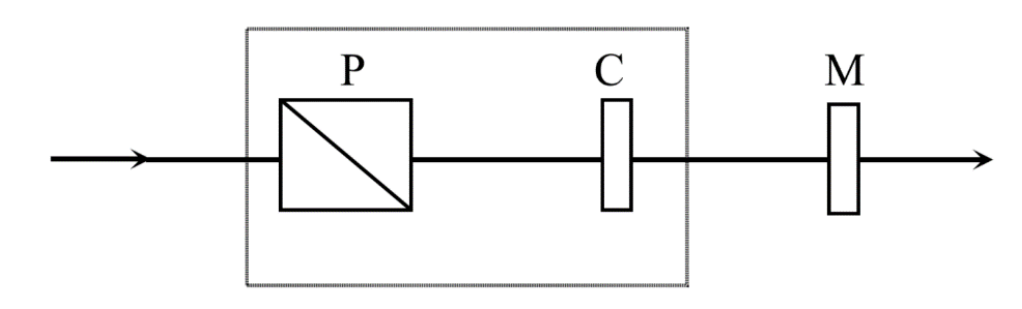
\includegraphics[width=0.6\textwidth]{img/optical_isolator.png}
    \caption{光隔离器示意图}
    \label{fig:optical_isolator}
\end{figure}

\textbf{位置关系:}波片快慢轴应与$P$透射轴成$45^{\circ}$

\textbf{原理:}

顺向行进的光被输入偏振片变成线偏振光(假设偏振方向为垂直)。接着, 1/4 波片会将光线的偏振方向旋转45度。最后,检偏器允许该光线通过该隔离器。

反向行进的光线则先通过1/4 波片,将该光线的偏振方向沿同一方向旋转45度。该光线最后会变成水平偏振。由于起偏器只允许垂直偏振光通过,故被阻隔。

\newpage
\section{教师签字的原始实验数据}

\begin{figure}[h]
    \centering
    \includegraphics[width=0.85\textwidth]{img/OriginalData1.jpg}
    \caption{原始实验数据1}
    \label{fig:raw_data_1}
\end{figure}

\begin{figure}[h]
    \centering
    \includegraphics[width=0.85\textwidth]{img/OriginalData2.jpg}
    \caption{原始实验数据2}
    \label{fig:raw_data_2}
\end{figure}

\begin{figure}[h]
    \centering
    \includegraphics[width=0.85\textwidth]{img/OriginalData3.jpg}
    \caption{原始实验数据3}
    \label{fig:raw_data_3}
\end{figure}

\end{document}
